\PassOptionsToPackage{table,xcdraw}{xcolor}
\documentclass[lettersize,journal]{IEEEtran}

% Include packages
%%%%%%%%%%%%%%%%%%%%%%%%%%%%%%%%%%%%%%%%%%%%%%%%%%%%%%%%%%%%%%%%%%%%%%%%%%%%%%%%
% In this file, only packages are allowed. These packages should be explained to
% greatest possible extent.
%%%%%%%%%%%%%%%%%%%%%%%%%%%%%%%%%%%%%%%%%%%%%%%%%%%%%%%%%%%%%%%%%%%%%%%%%%%%%%%%

% Document encodings
\usepackage[english]{babel}
\usepackage[utf8]{inputenc}
\usepackage[T1]{fontenc} % This can slightly change font appearance
\usepackage{xcolor} 

% Beamer theme
\usepackage{style/beamertheme} % Needes XeLaTeX

% Math related
\usepackage{amsmath, amssymb, amsthm, mathtools}
\usepackage{xfrac} %for nice inline fractions

% Char. related 
\usepackage{microtype}

% Bibliography related
\usepackage[backend=biber, style=authoryear]{biblatex}
\addbibresource{defence.bib}
\renewcommand*{\nameyeardelim}{\addcomma\space}
\AtBeginBibliography{\scriptsize}

%\usepackage{multirow} % For multirow tables
%\usepackage{colortbl} % For coloured tables

% Colordefinitions
\definecolor{misscolour}{RGB}{255, 0, 0}
\definecolor{lqrcolour}{RGB}{0,28,255}
\definecolor{lqrnomcolour}{RGB}{0,28,255}
\definecolor{lqgcolour}{RGB}{0,139,0}
\definecolor{lqgnomcolour}{RGB}{0,139,0}
\definecolor{adacolour}{RGB}{239,133,16}

\definecolor{baselinecolor}{rgb}{0.9, 0.78, 0.07}
\definecolor{markcolor}{rgb}{0.6, 0.64, 0.69}

\definecolor{hicolour}{RGB}{50, 50, 255}

% Tikz packages and related
\usepackage{tikz} 
\usepackage{pgfplots, pgfplotstable} 
\usepackage{fontawesome5} 

% Tikz Libraries
\usepgfplotslibrary{external}
    \tikzexternalize[prefix=tikz/]
    \tikzset{external/system call={lualatex \tikzexternalcheckshellescape
        -halt-on-error -interaction=batchmode -jobname "\image" "\texsource"}
    } % to let pdflatex work

\usepgfplotslibrary{groupplots}
\usepgfplotslibrary{fillbetween}
\pgfplotsset{colormap/viridis}
\pgfplotsset{compat=newest}
\usetikzlibrary{decorations.markings}
\usetikzlibrary{shapes}
\usetikzlibrary{backgrounds}
\usetikzlibrary{fit}

\usetikzlibrary{calc}
\usetikzlibrary{arrows}
\usetikzlibrary{arrows.meta}
\usetikzlibrary{patterns, patterns.meta}
\usetikzlibrary{shapes.misc}
%\pgfplotsset{compat=1.16}

%\usepgfplotslibrary{fillbetween}
\usetikzlibrary{positioning}
%\usepackage{makecell} 

%%% RTAS22B
\tikzset{Dom Node/.style={draw,
                        thick,
                        circle,
                        inner sep=0pt,
                        minimum size=12mm}%
}%
\tikzset{
    old inner xsep/.estore in=\oldinnerxsep,
    old inner ysep/.estore in=\oldinnerysep,
    Init Node/.style 2 args={draw,
                    thick,
                    circle,
                    minimum size=12mm,
                    old inner xsep=\pgfkeysvalueof{/pgf/inner xsep},
                    old inner ysep=\pgfkeysvalueof{/pgf/inner ysep},
                    /pgf/inner xsep=\oldinnerxsep+#1,
                    /pgf/inner ysep=\oldinnerysep+#1,
                    alias=sourcenode,
                    append after command={
                    let     \p1 = (sourcenode.center),
                            \p2 = (sourcenode.east),
                            \n1 = {\x2-\x1-#1-0.5*\pgflinewidth}
                    in
                        node [inner sep=0pt, draw, circle, minimum width=2*\n1,at=(\p1),#2] {}
                    }
    },
    Init Node/.default={2pt}{black}%
}%

%%% Comparison figure related
\def\xstart{1}
\def\xend{10} % change according to how many plots you have

% this is the list of styles
% define as many colours as the number of lines
% you could also change the marker etc
\pgfplotscreateplotcyclelist{blue10}{
    {blue!95!black, mark=*, mark size=2pt,mark options={fill=white}},
    {blue!85!black, mark=*, mark size=2pt},
    {blue!75!black, mark=*, mark size=2pt},
    {blue!65!black, mark=*, mark size=2pt},
    {blue!55!black, mark=*, mark size=2pt},
    {blue!45!black, mark=*, mark size=2pt},
    {blue!35!black, mark=*, mark size=2pt},
    {blue!25!black, mark=*, mark size=2pt},
    {blue!15!black, mark=*, mark size=2pt},
    {blue! 5!black, mark=*, mark size=2pt},
}

% argument #1: any options
\makeatletter
\newenvironment{customlegend}[1][]{%
    \begingroup
    % inits/clears the lists (which might be populated from previous
    % axes):
    \pgfplots@init@cleared@structures
    \pgfplotsset{#1}%
}{%
    % draws the legend:
    \pgfplots@createlegend
    \endgroup
}%

% makes \addlegendimage available (typically only available within an
% axis environment):
\def\addlegendimage{\pgfplots@addlegendimage}
\makeatother

%%% ECRTS 
\tikzset{cross/.style={%
    cross out,
    draw,
    minimum size=2*(#1-\pgflinewidth),
    inner sep=0pt, outer sep=0pt}}

\makeatletter
\pgfplotsset{
    every axis plot/.append style =
    {mark=none, mark options={fill=white}},
    mark max/.style={
        scatter/@pre marker code/.code={%
            \ifx\pgfplotspointmeta\pgfplots@metamax
                \def\markopts{}%
                \node [anchor=south, xshift=1mm, yshift=-0.4mm] { \pgfmathprintnumber[precision=1, fixed zerofill]{\pgfplotspointmeta} };
            \else
                \def\markopts{mark=none}
            \fi
                \expandafter\scope\expandafter[\markopts]
        },%
        scatter/@post marker code/.code={ \endscope },
        scatter
    }
}
% Style to select only points from #1 to #2 (inclusive)
\pgfplotsset{select coords between index/.style 2 args={
    x filter/.code={
        \ifnum\coordindex<#1\def\pgfmathresult{}\fi
        \ifnum\coordindex>#2\def\pgfmathresult{}\fi
    }
}}
\makeatother

\newcommand{\findmax}[1]{
    \pgfmathsetmacro\buffer{0.0}
    \pgfplotstableforeachcolumnelement{#1}\of\extdata\as\cellValue{%
        \pgfmathsetmacro{\buffer}{max(\buffer,\cellValue)}}
}
\newcommand*{\ReadOutElement}[4]{%
    \pgfplotstablegetelem{#2}{[index]#3}\of{#1}%
    \let#4\pgfplotsretval
}


% Include commands
%%%%%%%%%%%%%%%%%%%%%%%%%%%%%%%%%%%%%%%%%%%%%%%%%%%%%%%%%%%%%%%%%%%%%%%%%%%%%%%%
% In this file, only commands are allowed. These commands should be explained to
% greatest possible extent.
%%%%%%%%%%%%%%%%%%%%%%%%%%%%%%%%%%%%%%%%%%%%%%%%%%%%%%%%%%%%%%%%%%%%%%%%%%%%%%%%

%%% Blame commands
\newcommand{\pointout}[1]{\color{red}#1\color{black}} 

% Simplifying commands
\newcommand{\tool}{\texttt{\textbf{WeaklyHard.jl}}}
\newcommand{\toolL}{\texttt{\textbf{WHRTgraph}}}

% Maths general
\newcommand{\funof}[1]{\left( #1 \right)}
\newcommand{\abs}[1]{\left|#1\right|}
\newcommand{\norm}[1]{\left\lVert#1\right\rVert}
\DeclareMathOperator*{\argmax}{argmax}
\DeclareMathOperator*{\argmin}{argmin}
\newcommand{\nequiv}{\not\equiv}
\newcommand{\ourmod}[1]{\ \mathrm{mod}\ #1}
\newcommand{\tr}[1]{\mathrm{tr}\left(#1\right)} 

% Constraint names
\newcommand{\tAH}{\texttt{\textbf{AnyHit}}}
\newcommand{\tAM}{\texttt{\textbf{AnyMiss}}}
\newcommand{\tRH}{\texttt{\textbf{RowHit}}}
\newcommand{\tRM}{\texttt{\textbf{RowMiss}}}

% Constraints related
\newcommand{\anyhit}[1]{\binom{x_{#1}}{k_{#1}}}
\newcommand{\anymiss}[1]{\overline{\binom{x_{#1}}{k_{#1}}}}
\newcommand{\rowhit}[1]{\genfrac{<}{>}{0pt}{}{x_{#1}}{k_{#1}}}
\newcommand{\rowmiss}[1]{\overline{\genfrac{<}{>}{0pt}{}{x_{#1}}{k_{#1}}}}
\newcommand{\sset}[2]{\mathcal{S}_{#1}\funof{#2}}
\newcommand{\lweak}{\underline{\lambda}}
\newcommand{\lhard}{\overline{\lambda}}

\DeclarePairedDelimiter\ceil{\lceil}{\rceil}
\DeclarePairedDelimiter\floor{\left\lfloor}{\right\rfloor}

% Aliases in general
\newcommand{\strat}{\mathcal{H}} 
\newcommand{\LL}[1]{\mathcal{L}_{#1}} 
\newcommand{\overbar}[1]{\mkern 1.5mu\overline{\mkern-1.5mu#1\mkern-1.5mu}\mkern 1.5mu}

% Automaton related
\newcommand{\GG}[1]{\mathcal{G}_{#1}}                               % Automaton
\newcommand{\VV}[1]{V_{#1}}                                         % Nodes
\newcommand{\EE}[1]{E_{#1}}                                         % Edges
\newcommand*\BitAnd{\mathbin{\&}}
\newcommand*\BitOr{\mathbin{|}}
\newcommand*\ShiftLeft{\ll}
\newcommand*\ShiftRight{\gg}
\newcommand*\BitNeg{\ensuremath{\mathord{\sim}}}

% Figure related
\newcommand{\binsaggregatedhist}[0]{65}


% leave here for maths sloppiness
\sloppy

\begin{document}

\title{Stability of Linear Control Systems under Extended Weakly-Hard Constraints}

\author{Nils Vreman$^{1}$, Paolo Pazzaglia$^{2}$, Victor Magron$^{3}$, Jie Wang$^{3}$, Martina Maggio$^{2,1}$\\
$^{1}\,$Department of Automatic Control, Lund University, Sweden\\
$^{2}\,$Department of Computer Science, Saarland University, Germany\\
$^{3}\,$Laboratory for Analysis and Architecture of Systems, CNRS, France}
\author{Anonymous}

\markboth{IEEE Transactions on Computer-Aided Design of Integrated Circuits and Systems}%
{Stability of Linear Control Systems under Extended Weakly-Hard Constraints}

\maketitle

\begin{abstract}
Control systems can show robustness to many events, like disturbances and model inaccuracies.
It is natural to speculate that they are also robust to alterations of the control signal pattern, due to sporadic late completions (called \emph{deadline misses}) when implemented as a digital task on an embedded platform.
Recent research analysed stability when imposing constraints on the maximum number of consecutive deadlines that can be missed.
This is only one type of characterisation, and results in a pessimistic analysis when applied to more general cases.
To overcome this limitation, this paper proposes a comprehensive stability analysis for control systems subject to a set of generic constraints, describing the possible sequences  of correct completions and deadline misses.
The proposed analysis brings the assessment of control systems robustness to computational problems one step closer to the controller implementation.
\end{abstract}

\section{Introduction}
\label{sec:intro}
Robustness is an essential concern in the design of control systems; they must be able to reliably handle nonlinear effects, unmodeled dynamics and noise, as well as delays in signal transmissions and dropped packets.
A lesser known problem concerns the assessment of robustness to \emph{computational issues} when controllers are implemented as periodic tasks in cheap embedded platforms.
Such tasks are expected to execute with real-time guarantees, i.e., their execution must be completed before a well-defined \emph{deadline}, when the control output must be sent to the actuator.
However, it is common in practice~\cite{akesson2020empirical} that tasks do not always complete within their deadline, causing what is called a \emph{deadline miss}.
This may be caused by delays in computation and memory accesses, transient overloads, bugs and other issues.

A popular model to describe real-time systems allowing deadline misses is the \emph{weakly-hard} model~\cite{Bernat:2001}. 
Weakly-hard tasks feature constraints defining a maximum number of deadlines that can be missed (alternatively, a minimum number to be satisfied) in a given number of consecutive periods.
This model is also the focus of this work.
To analyse the effects on the controlled plant, it is necessary to specify also \emph{what happens when the miss is experienced}, both in terms of changes to the control signal and of actions taken to deal with the failed computation~\cite{Pazzaglia:2019}.
An instance that experiences a deadline miss can be allowed to continue executing until completion (and possibly used later), while in other applications it is stopped and discarded instead.

There is however a mismatch between the guarantees that can be obtained for real-time tasks and platforms~\cite{Ernst:2015,choi2019job}, and the analysis available for \emph{control} tasks under the weakly-hard model.
Fewer works deal with \emph{stability} analysis of weakly-hard real-time control tasks, often targeting specific use-cases. 
For instance, the analysis in~\cite{Maggio:2020} is limited to constraints specifying a maximum number of \emph{consecutive} deadline misses.
The results in \cite{Linsenmayer:2017,linsenmayer2020linear}, obtained for networked linear control systems having packet dropouts bounded using the weakly-hard model, can not be generalised for \emph{late completions} or \emph{sets} of weakly-hard constraints.
The authors of~\cite{liang2019security,liang2020leveraging} studied safety guarantees of weakly-hard controllers, considering a miss as a discarded computation with a known periodic pattern.
%
In \cite{huang2020saw, huang2019formal}, an over-approximation-based approach is proposed to check the safety of nonlinear weakly-hard systems, where misses are treated as discarded computations and the actuator holds its previous value.
Convergence rates (providing sufficient stability guarantees) are analysed in~\cite{Gaukler:2019a}.
A Lyapunov-based stability analysis of nonlinear weakly-hard systems is studied in~\cite{hertneck2021efficient}, with deadline misses treated as packet dropouts.
However, the state-of-the-art listed above lack generalisability to more expressive real-time implementations, such as different deadline miss models or handling strategies.

This paper aims at filling the gap, by providing a stability analysis that can be applied to a class of generic weakly-hard models and deadline miss handling strategies.
First, we formally extend the weakly-hard model to explicitly consider the strategy used to handle the miss events. 
By leveraging an automaton representation of the sequences allowed by (a set of) extended weakly-hard constraints, we use Kronecker lifting and the joint spectral radius to properly express its stability conditions.
Using the concept of constraint dominance, we prove analytic bounds on the stability of a weakly-hard system with respect to \emph{less dominant} constraints.
Finally, we analyse the stability of the resulting closed-loop systems using \code{SparseJSR}~\cite{sparsejsr}, which exploits the sparsity pattern that naturally arises in the Kronecker lifted representation.
The proposed analysis calls for modularity and separation of concern, and can be a useful tool to decouple the constraint specification and the control verification.
%, the embedded system designer can extract a set of constraints to be used in the design phase, and the control engineer can verify that the proposed constraints satisfy all control requirements. 


\section{Background and Notation}
\label{sec:background}
\chapter{Background}%
\label{ch:background}%

This chapter presents the necessary background and motivation for the remainder of the thesis.
We divide the chapter in two primary parts.
First, a discussion on the real-time theoretical aspects is provided.
An extended introduction to how real-time operating systems operates is presented, e.g., processor sharing, task states, scheduling strategies, etc.
However, the main focus is dedicated to the most commonly used task models and their respective advantages and disadvantages, with respect to deadline overruns.
Additionally, we provide a brief discussion on state-machine applicability to the aforementioned task models. 
Next, the relevant control theoretical background is presented based on the theory of real-time systems.
Two different system modelling approaches are introduced: switching systems and Markov jump linear systems.
Both models are particularly relevant for real-time systems where the control task can overrun its deadlines.
Specifically for these systems, we present and discuss different stability and performance analyses.

\section{Real-Time Systems}%
\label{sec:background:rts}%
%
% A short extension to the RTS (and RTOS) precise objective
We begin with an introduction to real-time system fundamentals. 
The breadth of the topic prevents a comprehensive review of the existing literature to fit within the scope of this thesis.
In fact, real-time systems are all information processing systems which takes external input and operate on it within a predetermined deadline. 
This includes sensors, actuators, process control, machine vision, robotics, and health care systems, to acknowledge a fraction of all real-time systems.
Instead, we focus the attention to the elements which impact real-time control systems the most, i.e., RTOS fundamentals, periodic tasks, task models, scheduling policies, and execution models.
\question%
{
    Maybe the ``RTOS fundamentals'' should be ``CPU provisioning'' and ``memory management'' instead?
}{}
Since the RTOS is tightly interconnected with the hardware, it is natural to illustrate them jointly.
In Figure~\ref{fig:operating-system-abstraction}, the underlying hardware and real-time structure is expanded.
%
\begin{figure}[t]
    \centering
    \def \delta {0.15}

\begin{tikzpicture}
\tikzstyle{task} = [draw,thick,fill=white,align=center]
\tikzstyle{circleconn} = [draw, fill=white, thick, circle, scale=0.5]

%%% TASKS %%%

\begin{scope}[on background layer]
    \node[task,opacity=0.3] (t1) at (-1.5+0*\delta,1.6-0*\delta) {\textcolor{white}{Task $\#3$} \\\textcolor{white}{\faFileCode[regular]}};
    \node[task,opacity=0.6] (t2) at (-1.5+1*\delta,1.6-1*\delta) {\textcolor{white}{Task $\#2$} \\\textcolor{white}{\faFileCode[regular]}};
    \node[task,opacity=1.0] (t3) at (-1.5+2*\delta,1.6-2*\delta) {Task $\#1$ \\\faFileCode[regular]};

    \node[task,opacity=0.3] (ct1) at (1+0*\delta,1.6-0*\delta) {\textcolor{white}{Control Task $\#3$} \\\textcolor{white}{\faFileCode[regular]}};
    \node[task,opacity=0.6] (ct2) at (1+1*\delta,1.6-1*\delta) {\textcolor{white}{Control Task $\#2$} \\\textcolor{white}{\faFileCode[regular]}};
    \node[task,opacity=1.0] (ct3) at (1+2*\delta,1.6-2*\delta) {Control Task $\#1$ \\\faFileCode[regular]};

    %%% CYBER %%%

    \node[thick, align=center] (rtos) at (-0.1,0.25) {Real-Time Operating System};
    \node[thick, draw, align=center, rotate=90, text width=2.75cm] (hwi) at (3.15,0.87) {HW Interfaces};
    \node[thick, fit=(rtos)(t1)(ct1)(ct3),draw,yshift=1.5mm,xshift=0.75mm] (sw) {};
    \node[thick, draw, above left] (clock) at (sw.south east) {\faClock[regular]};
    \node[thick, fit=(sw)(hwi), inner sep=7pt, draw] (hw) {};
    \node[thick, above left, xshift=2.3cm, yshift=0.5mm] (hw-label) at (hw.south west) {Hardware};
    \node[thick, draw, above right] (hwclock) at (hw.south west)  {\faClock[regular]};

    %%% PHYSICAL %%%

    \node[thick, draw ,align=center] (phys) at (6,0.87) {\includegraphics[scale=4]{\figdir/airplane.jpg}};
    \node[thick, draw, above left] (time) at (phys.south east) {\faClock[regular]};
\end{scope}


%%% ZOOM %%%

% Tasks
\node[task] (vt1) at (-0.9+0*10*\delta,1.0) {Task $\#1$ \\\faFileCode[regular]};
\node[task] (vt2) at (-0.9+1*10*\delta,1.0) {Task $\#2$ \\\faFileCode[regular]};
\node[]           at (-0.9+2*10*\delta,1.0) {$\cdots$};
\node[task] (vtn) at (-0.9+3*10*\delta,1.0) {Task $\#N$ \\\faFileCode[regular]};

\node[circleconn] (c1) at ($(vt1)+(0,-0.75)$) {};
\draw[thick] (c1.north) to (vt1.south);
\node[circleconn] (c2) at ($(vt2)+(0,-0.75)$) {};
\draw[thick] (c2.north) to (vt2.south);
\node[circleconn] (cn) at ($(vtn)+(0,-0.75)$) {};
\draw[thick] (cn.north) to (vtn.south);

% CPU
\node[task, minimum width=1.3cm, minimum height=1.0cm] (cpu) at (-0.9+1.5*10*\delta,-2.25) {CPU};

% Memory
\node[thick, draw, align=center, rotate=90, text width=2.25cm] (mem) at (-1.0+4*10*\delta,0.1) {Memory};

% HW interfaces
\node[thick, draw, align=center, rotate=90, text width=0.8cm] (gpio) at (-1.0+4*10*\delta,-2.15) {GPIO};

% Background 

\begin{scope}[on background layer]
    \node[thick, dashed, fill=white, fit=(vt1)(vtn)(cpu)(mem),draw,inner sep=4pt] (vhw) {};
    \draw[thick, dashed] ([yshift=-0.85cm]vhw.west) to ([yshift=-0.85cm]vhw.east);
    \draw[thick, dashed] ([xshift=2.65cm]vhw.south) to ([xshift=2.65cm]vhw.north);
\end{scope}

\draw[thick, dashed] (hw.south west) to (vhw.south west);
\draw[thick, dashed] (hw.north west) to (vhw.north west);
\draw[thick, dashed] (hw.north east) to (vhw.north east);

% Scheduler
\node[task, minimum width=5cm] (sched) at (-0.9+1.5*10*\delta,-1.0) {Scheduler};
\node[circleconn] (csched) at ($(sched)+(0,0.5)$) {};
\draw[thick] (csched.south) to (sched.north);

\draw[thick, -latex] (csched.north) to (c2.south);
\draw[thick, dashed, -latex, opacity=0.3] (csched.north) to (c1.south);
\draw[thick, dashed, -latex, opacity=0.3] (csched.north) to (cn.south);


\end{tikzpicture}
%
    \caption{\fix{Need to arrange figure so it makes more sense.}}%
    \label{fig:operating-system-abstraction}%
\end{figure}

% CPU, cores, and threads
The \emph{central processing unit} (CPU, or simply \emph{processor}) is the electronic component responsible for executing the task functions.
Each function (or program) is translated into a list of instructions to be executed on the CPU.
These instructions belong to the machine's language used to tell the processor what type of operation to execute, e.g., load a specific memory registry or execute an arithmetic operation.
To execute the program instructions, the processor can contain one or more \emph{cores}, respectively denoting the processor as \emph{single-core} or \emph{multi-core}.
Each core can execute a list of program instructions; hence, the advantage of using multi-core processors (compared to single-core processors) is the increased number of instructions that can be executed in parallel. 
However, this gain comes at the cost of an elevated system complexity where the memory and application layout has to be adapted to the multi-core architecture~\cite{Brandenburg:2011}.
\question{mention something about ``\#hardware threads = \#cores'' here?}{}

% Memory
Integrated with the processor is usually a \emph{cache} memory, i.e., a small but fast memory that is easy to access from the operational cores.
The cache memory stores recently accessed instructions and data to reduce the latency induced by fetching from main memory.
Most modern CPUs have a layered cache memory hierarchy, where the smallest and fastest layer is denoted L1, the second smallest and fastest is denoted L2, and so on.


% Tasks (Task stats, and states)
%

% Scheduler (how it allocates resources), mechanisms, deadline handling, many paragraphs here probably

% GPIO 
% describe scheduler, tasks, contexts, task states, etc.


\nv{Maybe create a figure with different task states?}

\subsection{Execution Modelling using State Machines}%
\label{sec:background:fsm}%
%


\section{Control Systems}%
\label{sec:background:ctrl}%
%

\subsection{Control System Stability}%
\label{sec:background:stability}%
%

\subsection{Control System Performance}%
\label{sec:background:performance}%
%


\nv{%

\section*{Embedded real-time control Systems}%
%
\begin{itemize}
    \item Refer to figure from Chapter~\ref{ch:intro} and then ``zoom'' in on the
        different aspects treated in the different subsections.
    \item Simple description of hardware components: Plant, Sensors, Network
        (wired/wireless), control hardware, actuators.
    \item Simple description of software components: network protocol, RTOS,
        tasks, memory, interrupts, etc.
    \item Maybe create a simple practical example (e.g., taxi of a plane) that
        can be followed throughout this section.
\end{itemize}


\subsection*{Real-Time Model}%
%
\begin{itemize}
    \item Start with a historical perspective
    \item Hard, Soft, Weakly-Hard, More expressive (\cite{Stigge:2011}), other?
    \item Describe advantages and disadvantages with each of the models
    \item recall great example of real-time system in rust book
\end{itemize}

\subsubsection*{Modelling Execution using finite state-machine}%
%
\begin{itemize}
    \item This section should maybe be moved?
    \item Entire subsubsection requested by KE
    \item More automata theory
    \item "typically in control fsm have been used to design highlevel control
        (e.g., taxi takeoff and landing), in principle (computer science)
        automata have been used to represent more complicated things (for
        instance regular languages). This is the basis of what the WeaklyHard.jl
        does."
    \item Include markov theory here. "In CS when the transition was
        non-deterministic, i.e., probabilistic, then you have the concept of
        Markov chains."
\end{itemize}


\subsection*{Control System Model}%
%
\begin{itemize}
    \item Start from plant, non-linear model, linearisation
    \item Sensors and actuator models included here.
    \item Control model (non-linear, more common ones), relate to real-time
        tasks
    \item Switching systems! Markov Jump Linear Systems!
\end{itemize}


\subsubsection*{Stability Analysis}%
%
\begin{itemize}
    \item Binary: Stable or not
    \item Stability definitions: nominal, MS, MSS, JSR, Lyapunov
    \item differences (e.g., JSR vs. Lyapunov), applicability
\end{itemize}


\subsubsection*{Performance Analysis}%
%
\begin{itemize}
    \item Gradient: varying degree of performance
    \item Why Performance Analysis?
    \item Metrics
\end{itemize}

}%


% MENTION SOMETHING ABOUT {SYNCHRONOUS, ASYNCHRONOUS, PERIODIC, APERIODIC} TASKS

% MENTION TASK STATES (INTERNAL AND EXTERNAL)


\section{Extended Weakly-Hard Task Model}
\label{sec:model}
To provide a comprehensive analysis framework, we need to examine what occurs in each time interval $(\pi_k)_{k \in \N_{\geq}}$, with $\pi_k = [a_0 + k\cdot \Ts, a_0 + (k+1)\cdot \Ts)$.
In this context, an extension of the weakly-hard model is required to account for the given deadline miss handling strategy, denoted with the symbol $\strat$.
%
\begin{definition}[Extended weakly-hard model $\tau \vdash \lambda^{\strat}$]%
    \label{def:new-mk}%
    A task $\tau$ may satisfy any combination of the four \emph{extended weakly-hard constraints} (\ewhc{}) $\lambda^{\strat}$:
    \begin{enumerate}[label=(\roman*)]
        \item $\tau \vdash \elcssanymiss{}{\strat}$: in any window of $\ell$ consecutive jobs, at most $x$ intervals lack a job completion;
        \item $\tau \vdash \elcssanyhit{}{\strat}$:  in any window of $\ell$ consecutive jobs, at least $x$ intervals have a job completion;
        \item $\tau \vdash \elcssrowmiss{}{\strat}$: in any window of $\ell$ consecutive jobs, at most $x$ \emph{consecutive} intervals lack a job completion;
        \item $\tau \vdash \elcssrowhit{}{\strat}$: in any window of $\ell$ consecutive jobs, at least $x$ \emph{consecutive} intervals have a job completion
    \end{enumerate}
    with $x\in \N_{\geq}$, $\ell \in \N_{>}$, and $x\leq \ell$, while using strategy $\strat$ to handle potential deadline misses.
\end{definition}
%
The definition above differs from the original weakly-hard model of~\cite{Bernat:2001}, since
\begin{enumerate*}[label=(\roman*)]
    \item it explicitly introduces the handling strategy $\strat$; and
    \item it focuses on the presence of a new control command at the end of each time interval $\pi_k$, instead of checking the deadline miss events, which guarantees its applicability also for strategies different than \tK{}.
\end{enumerate*}

We now require an expressive alphabet $\Sigma\left(\strat\right)$ to characterize the behaviour of task $\tau$ in each possible time interval.
For both \tK{} and \tS{} strategies, each interval $\pi_k$ contains at most one activated and one completed job.
This restricts the possible behaviours to three cases:
\begin{enumerate}[label=(\roman*)]
    \item a time interval in which the same job is both released and completed is denoted by $\cH$ (\emph{hit});
    \item a time interval in which no job is completed is denoted by $\cM$ (\emph{miss});
    \item a time interval in which no job is released, but a job (released in a previous interval) is completed, is denoted by $\cR$ (\emph{recovery}).
\end{enumerate}
%
By checking all unique combinations of job activations and completions in each interval, we obtain the alphabets for \tK{} and \tS{} as $\Sigma\left(\tK{}\right) = \{ \cM, \cH \}$ and $\Sigma\left(\tS{}\right) = \{ \cM, \cH, \cR \}$, respectively.
The recovery character $\cR$ is used in the \tS{} alphabet to identify the late \emph{completion} of a job.
As a consequence, $\cR$ is treated equivalently to $\cH$ when verifying the extended weakly hard constraints (\ewhc{}).


The algebra presented in Section~\ref{ssec:whalgebra} is extended to the new alphabet.
We assign a character of the alphabet $\Sigma\left(\strat\right)$ to each interval $\pi_k$.
A word $w = \seq{c_1,c_2,\dots,c_N}$ is used to represent a sequence of $N$ outcomes for task $\tau$, with $c_k \in \Sigma\left(\strat\right)$ representing the outcome associated to the interval $\pi_k$. 
To enforce only feasible sequences, we introduce an order constraint for the $\cR$ character with the following Rule.
%
\begin{rule_}[Outcome ordering]%
    \label{rule:R}%
    For any word $w \in \Sigma\left(\tS{}\right)^N$, $\cR$ may only directly follow $\cM$, or be the initial element of the word.
\end{rule_}

The extended weakly-hard model also inherits all the properties of the original weakly-hard model.
In particular, the satisfaction set of $\lambda^\strat$ can be defined for $N\geq 1$ as $\sset{N}{\lambda^{\strat}} = \{ w \in \Sigma\left(\strat\right)^N \mid w \vdash \lambda^{\strat} \}$, and the constraint domination still holds as $\lambda^{\strat}_{i} \preceq \lambda^{\strat}_{j}$ if $\sset{}{\lambda^{\strat}_{i}} \subseteq \sset{}{\lambda^{\strat}_{j}}$.


\section{State Machine Realisation}
\label{sec:state-machine}
In this section we propose a way to model a set of \ewhc{}, $\Lambda$, as an automaton, by utilising the satisfaction set $\sset{}{ \Lambda }$ and the concept of \emph{dominant set}.
The presented approach is invariant to the control system dynamics. 
For this reason, the resulting model can be used as an interface that separates the software design phase from the stability analysis (Section~\ref{sec:stability}), allowing the complete architecture analysis to be decoupled.

%\subsection{Constraint graph}%
%\label{sec:constraint_graph}
%%
%An \ewhc{}, as presented in Definition~\ref{def:new-mk}, can be systematically represented using an \emph{automaton} and the corresponding directed labeled graph.
%Each vertex in the graph corresponds to a subword of the last $k$ outcomes of the extended weakly-hard task executions. 
%Trivially, there exists no vertices for subwords that do not satisfy the \ewhc{}.
%A directed labeled edge connects two vertices if and only if the outcome $\event$ -- the edge's label -- appended to the tail vertex's subword representation would result in an equivalent one to the head vertex's.
%This implies that a random walk in the graph corresponds to a random word satisfying the \ewhc{}.
%Particularly, this implies that all the walks in the graph corresponds to \emph{all} words satisfying the \ewhc{}, i.e., $\sset{}{\lambda^{\strat}}$.
%
%\begin{figure}[t]
%    \begin{minipage}[c]{0.48\textwidth}
    \begin{center}
        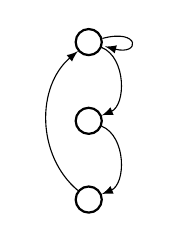
\begin{tikzpicture}[>=latex]
            \node[draw, thick, circle, radius=0.4] (a) at (0,0) {$\cX\cH\cH$};
            \node[draw, thick, circle, radius=0.4] (b) at (0,-1) {$\cH\cH\cM$};
            \node[draw, thick, circle, radius=0.4] (c) at (0,-2) {$\cH\cM\cH$};
            \draw[->] (a) edge [loop right] node[right] {$\cH$} (a);
            \draw[->] (a) edge [bend left=67.5] node[right] {$\cM$} (b);
            \draw[->] (b) edge [bend left=67.5] node[right] {$\cH$} (c);
            \draw[->] (c) edge [bend left=50] node[left] {$\cH$} (a);
        \end{tikzpicture}

        (Example~\ref{ex:auto-kill})\\[1pt]
        $\lambda^{\strat} = \overbar{\binom{1}{3}}^{\text{Kill}}$
    \end{center}
\end{minipage}
%
%    \begin{minipage}[c]{0.48\textwidth}
    \begin{center}
        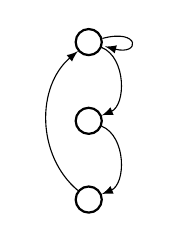
\begin{tikzpicture}[>=latex]
            \node[draw, thick, circle, radius=0.4] (a) at (0,0) {$\cX\cT\cH$};
            \node[draw, thick, circle, radius=0.4] (b) at (0,-1) {$\cT\cH\cM$};
            \node[draw, thick, circle, radius=0.4] (c) at (0,-2) {$\cH\cM\cR$};
            \draw[->] (a) edge [loop right] node[right] {$\cH$} (a);
            \draw[->] (a) edge [bend left=67.5] node[right] {$\cM$} (b);
            \draw[->] (b) edge [bend left=67.5] node[right] {$\cR$} (c);
            \draw[->] (c) edge [bend left=50] node[left] {$\cH$} (a);
        \end{tikzpicture}

        (Example~\ref{ex:auto-skip})\\[1pt]
        $\lambda^{\strat} = \overbar{\binom{1}{3}}^{\text{Skip-Next}}$
    \end{center}
\end{minipage}
%
%    \caption{Minimal graph $\GG{\lambda^{\strat}}^*$ for Examples 1 and 2.}
%    \label{fig:min-graph}
%\end{figure}
%
%We denote the graph corresponding to a task $\tau\vdash\lambda^{\strat}$ with the symbol $\GG{\lambda^{\strat}} = (\VV{\lambda^{\strat}}, \EE{\lambda^{\strat}})$.
%Here, $\VV{\lambda^{\strat}}$ represents the set of \emph{vertices} in the graph and $\EE{\lambda^{\strat}}$ represents the set of \emph{edges} (also denoted \emph{transitions}).
%Each vertex $v_i \in \VV{\lambda^{\strat}}$ corresponds to a word $\aword_i \in \sset{k}{\lambda^{\strat}}$.
%A \emph{subword} $\aword_i\left(a..b\right)$ of $\aword_i = \left\{ \event_1, \dots, \event_N \right\}$ is a new word containing the characters from position $a$ to position $b$, i.e., $\aword_i\left(a..b\right) = \left\{ \event_a, \dots, \event_b \right\}$.
%We use $\aword_i\left(a..\text{end}\right)$ to indicate the subword from position $a$ till the end of $\aword_i$.
%%
%A transition $e = (v_i,v_j,\event)\in \EE{\lambda^{\strat}}$, takes us from vertex $v_i$ to vertex $v_j$ and is labeled by the character $\event \in \Sigma\left(\strat\right)$.
%Vertex $v_j$ is said to be a direct successor of $v_i$ if concatenating the character $\event$ to the end of the vertex's word $\aword_i\left(2..end\right)$ gives $\aword_j$.
%
%Intuitively, a graph $\GG{\lambda^{\strat}}$ has \emph{at most} a number of vertices equal to the cardinality of the set of feasible words $\sset{k}{\lambda^{\strat}}$, or formally $\abs{\VV{\lambda^{\strat}}} \leq \abs{\sset{k}{\lambda^{\strat}}}$.
%However, to avoid unnecessary complexity, a \emph{minimal automaton} $\GG{\lambda^{\strat}}^*=(\VV{\lambda^{\strat}}^*, \EE{\lambda^{\strat}}^*)$ is easily obtained from $\GG{\lambda^{\strat}}$ using standard techniques~\cite{Hopcroft:2001}.
%Given two vertices $v_{i}$ and $v_{j}$, if they share the same successors with the same transition labels (i.e., outcomes) $\event$ they are considered equivalent and thereby combined.
%The differing characters in the word representations of $v_i$ and $v_j$ are replaced by an \emph{any outcome} token, which we denote with $\cX$.
%This process is repeated until the automaton can no longer be reduced.
%%
%When considering the Skip-Next strategy, an additional auxiliary token $\cT$ is introduced to represent all outcomes where a job is completed (ergo; $\cT = \left\{ \cH,\, \cR \right\}$).
%
%
%%\afterpage{%
%%    \clearpage
%    \begin{figure*}[h]
%        \begin{minipage}[c]{0.4\textwidth}
    \begin{center}
        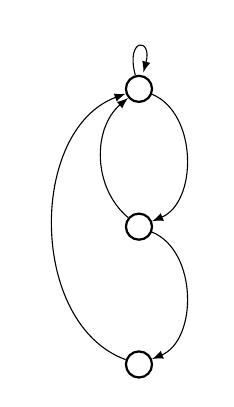
\begin{tikzpicture}[>=latex]
            \node[draw, thick, circle, radius=0.4] (a) at (0,0) {$\textcolor{white}{\cH}\cX\cX\cH\textcolor{white}{\cH}$};
            \node[draw, thick, circle, radius=0.4] (b) at (0,-1.75) {$\textcolor{white}{\cH}\cX\cH\cM\textcolor{white}{\cH}$};
            \node[draw, thick, circle, radius=0.4] (c) at (0,-3.5) {$\textcolor{white}{\cH}\cH\cM\cM\textcolor{white}{\cH}$};
            \draw[->] (a) edge [loop above] node[above] {$\cH$} (a);
            \draw[->] (a) edge [bend left=67.5] node[right] {$\cM$} (b);
            \draw[->] (b) edge [bend left=50] node[left] {$\cH$} (a);
            \draw[->] (b) edge [bend left=67.5] node[right] {$\cM$} (c);
            \draw[->] (c) edge [bend left=70] node[left] {$\cH$} (a);
        \end{tikzpicture}

        (Constraint 1)\\[1pt]
        $\lambda^{\strat}_1 = \overbar{\left<2\right>}^{\text{Kill}}$
    \end{center}
\end{minipage}
\hspace{1cm}
\begin{minipage}[c]{\textwidth}
    \begin{center}
        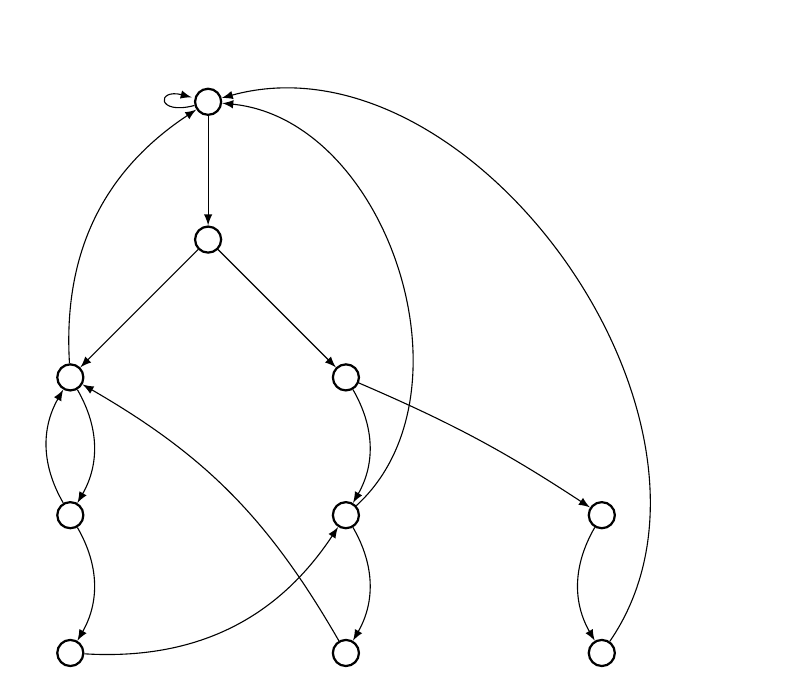
\begin{tikzpicture}[>=latex]
            \node[draw, thick, circle, radius=0.4] (a) at (0,0) {$\cX\cX\cX\cH\cH$};
            \node[draw, thick, circle, radius=0.4] (b) at (0,-1.75) {$\cX\cX\cH\cH\cM$};
            \node[draw, thick, circle, radius=0.4] (c) at (-1.75,-3.5) {$\cX\cX\cH\cM\cH$};
            \node[draw, thick, circle, radius=0.4] (d) at (-1.75,-5.25) {$\cX\cH\cM\cH\cM$};
            \node[draw, thick, circle, radius=0.4] (e) at (-1.75,-7) {$\cH\cM\cH\cM\cM$};
            \node[draw, thick, circle, radius=0.4] (f) at (1.75,-3.5) {$\cX\cH\cH\cM\cM$};
            \node[draw, thick, circle, radius=0.4] (g) at (1.75,-5.25) {$\cX\cH\cM\cM\cH$};
            \node[draw, thick, circle, radius=0.4] (h) at (1.75,-7) {$\cH\cM\cM\cH\cM$};
            \node[draw, thick, circle, radius=0.4] (i) at (5,-5.25) {$\cH\cH\cM\cM\cM$};
            \node[draw, thick, circle, radius=0.4] (j) at (5,-7) {$\cH\cM\cM\cM\cH$};

            \draw[->] (a) edge [loop left] node[left] {$\cH$} (a);
            \draw[->] (a) edge [] node[right] {$\cM$} (b);
            \draw[->] (b) edge node [above] {$\cH$} (c);
            \draw[->] (b) edge node [above] {$\cM$} (f);
            \draw[->] (c) edge [bend left] node [left] {$\cH$} (a);
            \draw[->] (c) edge [bend left] node [right] {$\cM$} (d);
            \draw[->] (d) edge [bend left] node [left] {$\cH$} (c);
            \draw[->] (d) edge [bend left] node [right] {$\cM$} (e);
            \draw[->] (e) edge [bend right] node [below] {$\cH$} (g);
            \draw[->] (f) edge [bend left] node [right] {$\cH$} (g);
            \draw[->] (f) edge [bend left=5] node [above] {$\cM$} (i);
            \draw[->] (g) edge [bend right = 66] node [right] {$\cH$} (a);
            \draw[->] (g) edge [bend left] node [right] {$\cM$} (h);
            \draw[->] (h) edge [bend right = 15] node [above] {$\cH$} (c);
            \draw[->] (i) edge [bend right] node [left] {$\cH$} (j);
            \draw[->] (j) edge [bend right = 70] node [right] {$\cH$} (a);

        \end{tikzpicture}

        (Constraint 2)\\[1pt]
        $\lambda^{\strat}_2 = \overbar{\binom{3}{5}}^{\text{Kill}}$
    \end{center}
\end{minipage}
\hspace{1cm}
\begin{minipage}[c]{0.8\textwidth}
    \begin{center}
        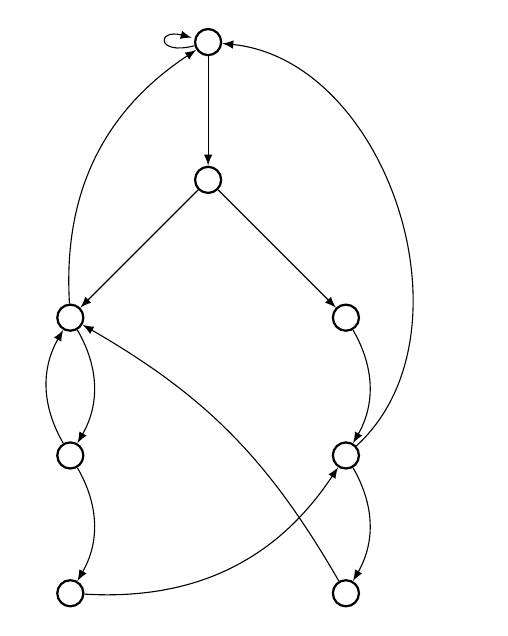
\begin{tikzpicture}[>=latex]
            \node[draw, thick, circle, radius=0.4] (a) at (0,0) {$\cX\cX\cX\cH\cH$};
            \node[draw, thick, circle, radius=0.4] (b) at (0,-1.75) {$\cX\cX\cH\cH\cM$};
            \node[draw, thick, circle, radius=0.4] (c) at (-1.75,-3.5) {$\cX\cX\cH\cM\cH$};
            \node[draw, thick, circle, radius=0.4] (d) at (-1.75,-5.25) {$\cX\cH\cM\cH\cM$};
            \node[draw, thick, circle, radius=0.4] (e) at (-1.75,-7) {$\cH\cM\cH\cM\cM$};
            \node[draw, thick, circle, radius=0.4] (f) at (1.75,-3.5) {$\cX\cH\cH\cM\cM$};
            \node[draw, thick, circle, radius=0.4] (g) at (1.75,-5.25) {$\cX\cH\cM\cM\cH$};
            \node[draw, thick, circle, radius=0.4] (h) at (1.75,-7) {$\cH\cM\cM\cH\cM$};

            \draw[->] (a) edge [loop left] node[left] {$\cH$} (a);
            \draw[->] (a) edge [] node[right] {$\cM$} (b);
            \draw[->] (b) edge node [above] {$\cH$} (c);
            \draw[->] (b) edge node [above] {$\cM$} (f);
            \draw[->] (c) edge [bend left] node [left] {$\cH$} (a);
            \draw[->] (c) edge [bend left] node [right] {$\cM$} (d);
            \draw[->] (d) edge [bend left] node [left] {$\cH$} (c);
            \draw[->] (d) edge [bend left] node [right] {$\cM$} (e);
            \draw[->] (e) edge [bend right] node [below] {$\cH$} (g);
            \draw[->] (f) edge [bend left] node [right] {$\cH$} (g);
            \draw[->] (g) edge [bend right = 66] node [right] {$\cH$} (a);
            \draw[->] (g) edge [bend left] node [right] {$\cM$} (h);
            \draw[->] (h) edge [bend right = 15] node [above] {$\cH$} (c);

        \end{tikzpicture}

        (Result)\\[1pt]
        $\Lambda^{\strat}_0 = \left\{ \lambda^{\strat}_1,\, \lambda^{\strat}_2 \right\}$
    \end{center}
\end{minipage}%}

%        \caption{Minimal graphs $\GG{\lambda^{\strat}_1}^*$, $\GG{\lambda^{\strat}_2}^*$, and $\GG{\Lambda^{\strat}_0}^*$ for Example~\ref{ex:auto-comb}.}
%        \label{fig:multi-graphs}
%    \end{figure*}
%%    \clearpage
%%}
%
%\begin{example}%
%    \label{ex:auto-kill}%
%    \emph{Given an \ewhc{},} $\lambda^{\strat} = \overbar{\binom{1}{3}}^{\text{Kill}}$\emph{, the minimal realisation $\GG{\lambda^{\strat}}^*$ is shown in the left-hand side of Figure~\ref{fig:min-graph}.
%    The vertex represented by the word $\cX\cH\cH$ is obtained by merging $\cH\cH\cH$ and $\cM\cH\cH$.}
%\end{example}
%
%\begin{example}%
%    \label{ex:auto-skip}%
%    \emph{Given an \ewhc{},} $\lambda^{\strat} = \overbar{\binom{1}{3}}^{\text{Skip-Next}}$\emph{, the minimal realisation $\GG{\lambda^{\strat}}^*$ is shown in the right-hand side of Figure~\ref{fig:min-graph}.}
%\end{example}
%
%The minimal automaton for Kill and Skip-Next in Figure~\ref{fig:min-graph} have identical number of vertices but slightly different transitions.
%This is not a coincidence, but follows directly from Definition~\ref{def:new-mk} and the extended alphabet $\Sigma\left(\strat\right)$.
%A hit ($\cH$) and a recovery ($\cR$) are both considered job completions, which is why the graphs for the Kill and Skip-Next strategies have the same structure.
%It is only the first job completion after a period of no job completions ($\cM$) that differ.
%However, the different transitions of the two graphs affect the corresponding closed-loop systems, as will be clear in Section~\ref{sec:stability}.
%
%\subsection{Dealing with multiple constraints}
%\label{sec:mult-const}
%
%The approach presented above for constructing a minimal automaton can be extended to the case where the task $\tau$ is subject to a set of multiple \ewhc{}. 
%Such a set is formally denoted as $\Lambda^{\strat}$.
%%
%In order to optimise the problem of building the minimal automaton of the corresponding system, it is beneficial that the set $\Lambda^{\strat}$ contains only constraints that cannot be further reduced using the hardness relations of Definition~\ref{def:domination}. 
%To this end, we first introduce the new concept of \emph{dominant (constraint) set}.
%%
%\begin{definition}[Dominant set]%
%    \label{def:dominant-set}%
%    %
%    Given a set of \ewhc{}, $\Lambda^{\strat}$, the set $\Lambda^{\strat}_0 \subseteq \Lambda^{\strat}$ is called the \emph{dominant set} of $\Lambda^{\strat}$ if:
%    \begin{enumerate}[label=(\roman*)]
%        \item $\lambda^{\strat}_i,\lambda^{\strat}_j \in \Lambda^{\strat}_0 \,\,\implies \lambda^{\strat}_i \npreceq \lambda^{\strat}_j,\, \forall i \neq j,$
%        \item $\lambda^{\strat}_i \in \Lambda^{\strat} \setminus \Lambda^{\strat}_0 \implies
%            \lambda^{\strat}_j \preceq \lambda^{\strat}_i,\, \exists \lambda^{\strat}_j \in \Lambda^{\strat}_0.$
%    \end{enumerate}
%\end{definition}
%
%Building upon Definition~\ref{def:satisfaction}, the satisfaction set of $\Lambda^{\strat}_0$ can be derived as follows, for $N\geq 1$:
%%
%\begin{equation}
%    \label{eq:satisfaction-multi}
%    \sset{N}{\Lambda^{\strat}_0} \equiv \bigcap_{\lambda^{\strat}_i \in \Lambda^{\strat}_0} \sset{N}{\lambda^{\strat}_i}.
%\end{equation}
%%
%We can then obtain a minimal graph $\GG{\Lambda^{\strat}_0}^*$ following a procedure similar to the one presented for a single constraint $\lambda^{\strat}$ in Section~\ref{sec:state-machine}.
%As a first step, the length of the words in each vertex of the corresponding graph must be defined.
%Since $\Lambda^{\strat}_0$ may contain constraints with different window values, the choice is not straightforward.
%We propose a safe assumption about the word length $k_0$, defined as $\,k_0 = \max_{k} \lambda^{\strat},\,\, \forall \lambda^{\strat} \in \Lambda^{\strat}_0$.
%An algorithm can then be built that adds vertices, with word representations $\aword_i \in \sset{k_0}{ \Lambda^{\strat}_0 }$, to the graph until a minimal realisation is generated.
%The obtained graph is finally passed through a post-processing step (strategy-dependent) that assigns the appropriate transitions in order to obtain a correct minimal automaton realisation $\GG{\Lambda^{\strat}_0}^*$.
%
%\begin{example}%
%    \label{ex:auto-comb}%
%    \emph{Given two \ewhc{},} $\lambda^{\strat}_1 = \overbar{\left<2\right>}^{\text{Kill}}$\emph{ and } $\lambda^{\strat}_2 = \overbar{\binom{3}{5}}^{\text{Kill}}$\emph{, the minimal realisation graphs $\GG{\lambda^{\strat}_1}^*$ and $\GG{\lambda^{\strat}_2}^*$ are shown as the leftmost and middle graphs of Figure~\ref{fig:multi-graphs}.
%    Generating the graph $\GG{\Lambda^{\strat}_0}^*$ from the dominant set $\Lambda^{\strat}_0 = \{ \lambda^{\strat}_1, \lambda^{\strat}_2 \}$ results in the rightmost graph of Figure~\ref{fig:multi-graphs}, satisfying both $\lambda^{\strat}_1$ and $\lambda^{\strat}_2$.}
%\end{example}
%
%
%Building a minimal automaton by choosing the dominant set $\Lambda^{\strat}_0$ improves the computational performance of the analysis.
%Nonetheless, the analysis presented in the following sections can be applied to any graph built from a given set $\Lambda^{\strat}$.
%To limit complexity in the notation, and for the sake of generality, all future steps will consider a generic graph $\GG{\Lambda^{\strat}}=(\VV{\Lambda^{\strat}}, \EE{\Lambda^{\strat}})$.
%
%
%\subsection{Dynamic model of a graph}
%\label{ssec:dynamicgraph}
%
%Extracting all the transitions in $\EE{\Lambda^\strat}$ corresponding to a character $\event$ yields what is generally known as a \emph{directed adjacency matrix}~\cite{xu2012matrix}, denoted here as a \emph{transition matrix}.
%\begin{definition}[Transition matrix]
%    \label{def:transition}
%    Given a graph $\GG{\Lambda^\strat}$, the \emph{transition matrix} $F_{\event} ( \GG{\Lambda^\strat} ) \in \R^{\abs{\VV{\Lambda^\strat}} \times \abs{\VV{\Lambda^\strat}}}$ with $\event\in\Sigma\left(\strat\right)$, is computed as $F_{\event} ( \GG{\Lambda^\strat} ) = \{f_{i,j}(\event)\}$ with
%    %
%    \begin{equation*}
%        f_{i,j}\funof{\event}=
%        \begin{cases}
%            1, &\text{ if } \exists \, e=(v_j,v_i,\event) \in \EE{\Lambda^\strat} \\
%            0, &\text{ otherwise.}
%        \end{cases}
%        \end{equation*}%
%\end{definition}
%%
%Since there can only exist \emph{at most one} successor from each vertex with a transition labeled with $\event$, the transition matrix $F_\event$ will thus have a column sum of either 1 or 0.
%We introduce a vector $q_t\in \R^{\abs{\VV{\Lambda^\strat}}}$ called \emph{G-state} (for graph state), representing the state of the given graph $\GG{\Lambda^\strat}$, which is associated to the interval $\pi_t$.
%This vector is formally defined as follows.
%\begin{definition}[G-state $q_t$]\label{def:qt}
%    Given a graph $\GG{\Lambda^\strat} = (\VV{\Lambda^\strat}, \EE{\Lambda^\strat})$ and a sequence $\aword \in \Sigma\left( \strat \right)^N$, for $k = \abs{v},\,\, v\in\VV{\Lambda^\strat}$, we define $q_t\in \R^{\abs{\VV{\Lambda}}}$, where the $i$-th element $q_{t,i}$ is defined as:
%    \begin{equation*}
%        q_{t,i}=
%        \begin{cases}
%            1, &\text{ if } \aword\left(t-k..t-1\right) \equiv v_i \in \VV{\Lambda^\strat} \\
%            0, &\text{otherwise}.
%        \end{cases}
%    \end{equation*}
%\end{definition}
%In other words, the G-state $q_t$ is the vector representation of the vertex we are \emph{leaving} at step $t$.
%In this definition, $q_t=0$ means that the transition at step $t-1$ was infeasible for the graph.
%The G-state dynamics, given an arbitrary sequence $\aword=\{\alpha_1,\dots,\alpha_t,\dots,\}$, is then defined as $q_{t+1} = F_{\event} ( \GG{\Lambda^\strat} )\cdot q_t$.
%Hence, the following property from~\cite{xu2012matrix} holds.
%\begin{lemma}[Infeasible sequence]
%    \label{cor:Fseqnotinlambda}
%    If $\aword \notin \sset{N}{ \Lambda^\strat }$, then $F_{\aword} ( \GG{\Lambda^\strat} ) =
%    F_{\event_N} ( \GG{\Lambda^\strat} )\cdots F_{\event_2} ( \GG{\Lambda^\strat} )\cdot F_{\event_1} ( \GG{\Lambda^\strat} ) = 0$
%\end{lemma}
%Thus, if $q_t=0$ for any $t$, then $q_{t'}=0$ for $t' \geq t$.


\section{Stability Analysis}
\label{sec:stability}
Using the alphabet $\Sigma\left(\strat\right)$ and the chosen actuator mode (i.e., \tZ{}ing, or \tH{}ing the previous value), we compute the closed-loop behaviour of the controlled system.
We identify one matrix for each dynamics corresponding to an interval $\pi_k$ associated by $c \in \Sigma\left( \strat \right)$, building the set $\Aa^\strat$.

\textbf{\tK{}: }%
%
Defining $\tilde x_k^{\,\Kill} = \left[ x_k^\T{}\,\, z_k^\T{}\,\, u_k^\T{} \right]^\T{}$ as the closed-loop state vector,
we compute the discrete time closed-loop system dynamics $\clmat{}^{\,\Kill}_{\cH}$, corresponding to the character $\cH$:
\begin{equation*}
    \tilde x_{k+1}^{\,\Kill} = \clmat{}^{\,\Kill}_{\cH}\,\tilde x_k^{\,\Kill}, \quad\;
     \clmat{}^{\,\Kill}_{\cH} = \begin{bmatrix}
        \Ap       & 0    & \Bp       \\
        -\Bc\Cp   & \Ac  & -\Bc\Dp   \\
        -\Dc\Cp   & \Cc  & -\Dc\Dp   \\
    \end{bmatrix}.
\end{equation*}
%
For the case of $\cM$, the controller execution terminates prematurely and its states are not updated ($z_{k+1} = z_k$).
Therefore, depending on the actuation mode (\tZ{} or \tH{}), the controller output is either zeroed ($u_{k+1} = 0$) or held ($u_{k+1} = u_k$).
The resulting closed-loop system in state-space form is denoted with $\clmat{}^{\,\Kill}_{\cM}$:
\begin{equation*}
    \tilde x_{k+1}^{\,\Kill} = \clmat{}^{\,\Kill}_{\cM}\,\tilde x_k^{\,\Kill}, \quad
   \clmat{}^{\,\Kill}_{\cM} = \begin{bmatrix}
        \Ap & 0  & \Bp \\
        0   & I  & 0   \\
        0   & 0  & \Delta
    \end{bmatrix}.
\end{equation*}
Here, $\Delta = I$ (identity matrix) if the control signal is held and $\Delta = 0$ if zeroed.
The set of dynamic matrices under the \tK{} strategy is then $\Aa^{\,\Kill}=\left\{\clmat{}^{\,\Kill}_{\cH},\clmat{}^{\,\Kill}_{\cM}\right\}$.

\textbf{\tS{}: }%
%
For the \tS{} strategy, we introduce two additional states $\hat x_k$ and $\hat u_k$ storing the old values of $x_k$ and $u_k$ while the controller awaits an update.
The resulting state vector then becomes $\tilde x_k^{\,\Skip} = \left[ x_k^\T{}\,\,z_k^\T{}\,\, u_k^\T{}\,\, \hat{x}_k^\T{}\,\, \hat{u}_k^\T{} \right]^\T{}$.
When $\pi_k$ is associated to $\cH$, the two additional states mirror the behaviour of the states of which they are storing data.
The resulting closed-loop system is described using $\clmat{}^{\,\Skip}_{\cH}$:
\begin{equation*}
    \setlength\arraycolsep{3pt}
    \tilde x_{k+1}^{\,\Skip} = \clmat{}^{\,\Skip}_{\cH}\,\tilde x_k^{\,\Skip}, \quad
    \clmat{}^{\,\Skip}_{\cH} = \begin{bmatrix}
        \Ap       & 0    & \Bp      & 0 & 0 \\
        -\Bc\Cp   & \Ac  & -\Bc\Dp  & 0 & 0 \\
        -\Dc\Cp   & \Cc  & -\Dc\Dp  & 0 & 0 \\
        \Ap       & 0    & \Bp      & 0 & 0 \\
        -\Dc\Cp   & \Cc  & -\Dc\Dp  & 0 & 0 \\
    \end{bmatrix}.
\end{equation*}
%
For the case of $\cM$ in $\pi_k$, $\hat x_k$ and $\hat u_k$ maintain their previous values. The
resulting closed-loop is described by $\clmat{}^{\,\Skip}_{\cM}$:
%
\begin{equation*}
    \setlength\arraycolsep{3pt}
    \tilde x_{k+1}^{\,\Skip} = \clmat{}^{\,\Skip}_{\cM}\,\tilde x_k^{\,\Skip}, \quad
    \clmat{}^{\,\Skip}_{\cM}=\begin{bmatrix}
        \Ap & 0  & \Bp & 0 & 0 \\
        0   & I  & 0   & 0 & 0 \\
        0   & 0  & \Delta   & 0 & 0 \\
        0   & 0  & 0   & I & 0 \\
        0   & 0  & 0   & 0 & I \\
	\end{bmatrix}.
\end{equation*}
%
Finally, for the case of $\cR$, the new control command is calculated using the values stored in $\hat x_k$ and $\hat u_k$.
The resulting closed-loop system is described by $\clmat{}^{\,\Skip}_{\cR}$:
%
\begin{equation*}
    \setlength\arraycolsep{3pt}
    \tilde x_{k+1}^{\,\Skip} = \clmat{}^{\,\Skip}_{\cR} \, \tilde x_{k}^{\,\Skip},\quad
    \clmat{}^{\,\Skip}_{\cR} = \begin{bmatrix}
        \Ap & 0    & \Bp & 0       & 0 \\
        0   & \Ac  & 0   & -\Bc\Cp & -\Bc\Dp \\
        0   & \Cc  & 0   & -\Dc\Cp & -\Dc\Dp \\
        \Ap & 0    & \Bp & 0       & 0 \\
        0   & \Cc  & 0   & -\Dc\Cp & -\Dc\Dp \\
    \end{bmatrix}.
\end{equation*}
%
The resulting set of matrices under the \tS{} strategy is then defined as $\Aa^{\,\Skip}=\left\{\clmat{}^{\,\Skip}_{\cH},\clmat{}^{\,\Skip}_{\cM},\clmat{}^{\,\Skip}_{\cR}\right\}$.


\subsection{Kronecker lifted switching system}%
\label{sec:system_dynamics}

Combining the set of system dynamics $\Aa^\strat$ with the associated automaton $\GG{\Lambda^\strat}$, we seek to obtain an equivalent system model based on Kronecker lifting, characterized by a set of matrices denoted by $\Alifted_{\Lambda^\strat}$ and behaving as an \emph{arbitrary switching system}, such that $\rho\,(\Alifted_{\Lambda^\strat})= \rho\,(\Aa^{\strat},\GG{\Lambda^\strat})$.
In this way, powerful algorithms applicable to arbitrary switching system~\cite{vankeerberghen2014jsr,sparsejsr} can be used to find tight stability bounds.
%
We build upon the Kronecker lifting approach of~\cite{xu2020approximation}.
Leveraging the vector $q_k$ of Definition~\ref{def:qt}, we introduce the \emph{lifted discrete-time state} $\xi_k \in \R^{n\cdot n_V}$, defined as $\xi_k = q_k\otimes x_k$, where $n_V = \abs{\VV{\Lambda^\strat}}$ and $\otimes$ is the Kronecker product.
By construction, $\xi_k$ is a vector composed of $n_V$ blocks of size $n$, where at most one block is equal to $x_k$ and all other blocks are equal to the $0$ vector.
%
Then, we build a set of lifted matrices $L_{c} ( \GG{\Lambda^\strat} ) \in \R^{n\cdot n_V\times n\cdot n_V}$, which incorporates both the system dynamics and the possible transitions given a certain outcome $c\in\Sigma\left(\strat\right)$:
%
\begin{equation}\label{eq:lifted_matrix}
    L_{c} ( \GG{\Lambda^\strat} ) = F_{c} ( \GG{\Lambda^\strat} )\otimes \clmat^\strat_c, \quad c \in \Sigma \left( \strat \right).
\end{equation}
%
The lifted dynamics of the closed loop system then become $ \xi_{k+1} = L_{c} ( \GG{\Lambda^\strat} )\cdot\xi_k.  $
Formally, we obtain a system composed of a set of switching dynamic matrices, $\Alifted_{\Lambda^\strat}$.
%
\begin{definition}[Lifted switching set $\Alifted_{\Lambda^\strat}$]%
    \label{def:switching_set}%
    Given a set of dynamic matrices $\Aa^{\strat}$ and an automaton $\GG{\Lambda^\strat}$, the switching set $\Alifted_{\Lambda^\strat}$ is defined as:
    $$
        \Alifted_{\Lambda^\strat} = \left\{ L_{c} ( \GG{\Lambda^\strat} ) \,\, | \,\, c \in \Sigma\left(\strat\right) \right\}.
    $$
\end{definition}%
%
Leveraging the mixed-product property of $\otimes$ and introducing a proper submultiplicative norm, it is possible to prove that $\rho\left(\Alifted_{\Lambda^\strat}\right)= \rho\,(\Aa^{\strat},\GG{\Lambda^\strat})$.
For more details and a formal proof we refer the interested reader to~\cite{xu2020approximation}.

\subsection{Extended weakly hard and JSR properties}
\label{sec:analytic_results}
We now provide a general relation between \emph{all} \ewhc{}s in terms of the joint spectral radii.
%
\begin{theorem}[JSR dominance]
    \label{th:rho_dominance_general}
    Given $\lambda_1^\strat$ and $\lambda_2^\strat$ as arbitrary \ewhc{}s, if $\lambda_2^\strat \preceq \lambda_1^\strat$ then
    $$
        \rho\funof{\Alifted_{\lambda_2^\strat}} \leq \rho\funof{\Alifted_{\lambda_1^\strat}}.
    $$
%
    \begin{proof}
        From Equation~\eqref{jsr}, for a generic \ewhc{} $\lambda^\strat$,
        \begin{equation*}
            \rho\left(\Alifted_{\lambda^\strat}\right) = \lim_{\ell\rightarrow \infty} \rho_\ell \left(\Alifted_{\lambda^\strat}\right), \;\, 
            \rho_\ell\left(\Alifted_{\lambda^\strat}\right) = \max_{a \in \sset{\ell}{\lambda^\strat}}\norm{\clmat_{a}}^{1/\ell}.
        \end{equation*}
        Definition~\ref{def:domination} gave us that $\lambda^\strat_2 \preceq \lambda^\strat_1$ iff $\sset{}{\lambda^\strat_2} \subseteq \sset{}{\lambda^\strat_1}$.
        Thus, if for a word $b$ it holds that $b \in \sset{\ell}{\lambda^\strat_2}$, then it also holds that $b \in \sset{\ell}{\lambda^\strat_1}$.
        The set of all possible $\clmat_{b}$ is thus included in the set of all possible $\clmat_{a},\, a \in \sset{\ell}{\lambda^\strat_1}$, thus:
        \begin{equation*}
            \max_{b \in \sset{\ell}{\lambda^\strat_2}}\norm{\clmat_{b}}^{1/\ell} \leq
            \max_{a \in \sset{\ell}{\lambda^\strat_1}}\norm{\clmat_{a}}^{1/\ell}, \quad \forall \ell \in \N_{>}.
        \end{equation*}
        The theorem follows immediately when $\ell\rightarrow \infty$.
    \end{proof}
\end{theorem}
%
Theorem~\ref{th:rho_dominance_general} is the first result that provides an analytic, correlation between the control theoretical analysis and real-time implementation.
Primarily, it implies that the constraint dominance from Definition~\ref{def:domination} also carries on to the JSR, giving us a notion of \emph{JSR dominance}.
The results of Theorem~\ref{th:rho_dominance_general} are strategy-independent, further reducing the coupling between the control analysis and real-time implementation, and are also independent of the controlled system's dynamics.

Two Corollaries of Theorem~\ref{th:rho_dominance_general} are derived for the commonly used models $\erowmiss{}{\strat}$ and $\eanymiss{}{\strat}$, highlighting some practical relations between such constraints.
\begin{corollary}[$\eanymiss{}{\strat}$ dominance]%
    \label{cor:rho_dominance_mk}%
    Given $\lambda^\strat_1 = \overbar{\binom{x}{k_1}}^{\strat}$ and $\lambda^\strat_2 = \overbar{\binom{x}{k_2}}^{\strat}$, if $k_1 \leq k_2$ then
    $$
        \rho\funof{\Alifted_{\lambda^\strat_2}} \leq \rho\funof{\Alifted_{\lambda^\strat_1}}.
    $$
\end{corollary}
\begin{corollary}[$\erowmiss{}{\strat}$ dominance]%
    \label{cor:rho_dominance_cons}%
    Given $\lambda^\strat_1 = \erowmiss{}{\strat}$ and $\lambda^\strat_2 = \eanymiss{}{\strat}$, then
    $$
        \rho\funof{\Alifted_{\lambda^\strat_2}} \leq \rho\funof{\Alifted_{\lambda^\strat_1}}.
    $$
\end{corollary}
%
The conclusions drawn from Theorem~\ref{th:rho_dominance_general} are theoretical, but its practical applicability lies in the algorithm used to find $\rho^{LB}$ and $\rho^{UB}$, i.e., lower and upper bounds for the JSR value.
Using these bounds we can determine the stability of the corresponding switching systems, as follows:
%
$$
\rho^{LB} \funof{ \Alifted_{\lambda^\strat_2} } \leq \rho \funof{ \Alifted_{\lambda^\strat_2} } \leq \rho \funof{ \Alifted_{\lambda^\strat_1} } \leq \rho^{UB} \funof{ \Alifted_{\lambda^\strat_1} }.
$$
%
Regardless of the algorithm used to find the bounds, if $\lambda^\strat_2 \preceq \lambda^\strat_1$ and $\rho^{UB} ( \Alifted_{\lambda^\strat_1} ) < 1$, the system under $\lambda^\strat_2$ is switching stable.
A similar relation holds for the lower bound.

Theorem~\ref{th:rho_dominance_general} can be further extended by relating the joint spectral radius of a single constraint to sets of constraints.
\begin{theorem}%
    \label{th:rho_dominance_set_general}%
    Given an arbitrary \ewhc{} $\lambda^\strat$, it holds that
    $$
        \rho\left(\Alifted_{\Lambda^\strat}\right) \leq \rho \left( \Alifted_{\lambda^\strat} \right) ,\,\, \forall \Lambda^\strat \ni \lambda^\strat.
    $$
    \begin{proof}
        For an arbitrary \ewhc{} set $\Lambda^\strat = \{\lambda^\strat_1, \dots, \lambda^\strat_N\}$, its satisfaction set is
        $$
            \sset{\ell}{\Lambda^\strat} = \bigcap_{i \in \{1,\dots, N\}} \sset{\ell}{\lambda^\strat_i}.
        $$
        Thus, for any $\lambda^\strat_i \in \Lambda^\strat$ it holds that 
        $$
            \sset{\ell}{ \Lambda^\strat } \subseteq \sset{\ell}{\lambda^\strat}.
        $$
        If a word $b$ is in $\sset{\ell}{\Lambda^\strat}$ it also belongs to $\sset{\ell}{\lambda^\strat}$. 
        The set of all possible $\clmat_{b}$ is thus included in the set of all possible $\clmat_{a},\, a \in \sset{\ell}{\lambda^\strat}$.
        As a consequence it holds that
        \begin{equation*}
            \max_{b \in \sset{\ell}{\Lambda^\strat}} \norm{\clmat_{b}}^{1/\ell} \leq
            \max_{a \in \sset{\ell}{\lambda^\strat}} \norm{\clmat_{a}}^{1/\ell}, \quad
            \forall \ell \in \N_{>}.
        \end{equation*}
        The theorem follows immediately when $\ell\rightarrow \infty$.
    \end{proof}
\end{theorem}

As in Theorem~\ref{th:rho_dominance_general}, the more we restrict the execution pattern of the control task with sets of constraints, the lower its JSR will be.
%
Theorem~\ref{th:rho_dominance_set_general} delivers the practical insight that enforcing tighter \ewhc{} to a stable system will \emph{never} destabilise it, as formally stated in the following corollary.
\begin{corollary}%
    \label{cor:rho_dominance_set}%
    Given an arbitrary \ewhc{} $\lambda^\strat$, if $\rho \left( \Alifted_{\lambda^\strat} \right) < 1$ then
    $$
        \rho\left(\Alifted_{\Lambda^\strat}\right) < 1 ,\,\, \forall \Lambda^\strat \ni \lambda^\strat.
    $$
\end{corollary}


\section{Evaluation}
\label{sec:evaluation}
We now apply the lifted dynamics model presented in Section~\ref{sec:stability} to two representative case studies.
The corresponding controllers are designed to stabilise the closed loop in ideal conditions, i.e., without deadline misses.
Numerical experiments are performed to analyse the stability of the control systems subject to different constraints, particularly the $\eanymiss{}{\strat}$ constraints.
We consider all combinations of strategy (\tK{} or \tS{}) and actuator mode (\tZ{} or \tH{}).

For each combination of control system and \ewhc{}, $\lambda^{\strat}$, the lifted set $\Alifted_{\lambda^\strat}$ is generated.
We approximate the JSR of $\Alifted_{\lambda^\strat}$ using three different algorithms.
First, a lower and upper bound of $\rho \left( \Alifted_{\lambda^\strat} \right)$ are computed using the \code{JSR toolbox}~\cite{vankeerberghen2014jsr}.
We compare these bounds with an upper bound of the JSR obtained via SOS relaxations, described in Section~\ref{sec:existing}; both the \emph{dense} and \emph{sparse} algorithm from the \code{SparseJSR} toolbox~\cite{sparsejsr} are executed, obtaining $\rho_{\sos,2d}\left(\Alifted_{\lambda^\strat}\right)$ and $\rho_{\textrm{TSSOS},2d}\left(\Alifted_{\lambda^\strat}\right)$ respectively.
%
For efficiency, we run experiments at the first relaxation order $d = 1$.

The \code{JSR toolbox} provides an accurate lower bound and a coarse upper bound in a few seconds.
In contrast, the dense SOS-based method usually finds a good upper bound but takes more time.
The sparse/dense upper bounds are obtained with the \code{SparseJSR} Julia package.
Since \code{JSR toolbox} and \code{SparseJSR} are implemented in different programming languages (Matlab and Julia) and rely on different SDP solvers (SDPT3/SeDuMi and MOSEK), it is not meaningful to compare their respective timings.
However, the time it takes to run the dense and sparse SOS methods in Julia is compared.
All numerical examples have been computed on an Intel Core i5-8265U@1.60GHz CPU with 8GB RAM memory.

\subsection{Process Industrial Plant}\label{sec:eval:stable}
We here analyse a stable discrete-time plant $\plant_1$, representative of the process industry~\cite{Hagglund:2002}, controlled using a PI-controller $\ctrler_1$ (sampled using the sampling period $\Ts = 0.5$~s):
\begin{equation*}
    %plant = batch 4, ID 1
    \plant_1: \,\, \left\{
    \begin{aligned}
        x_{k+1} &= \begin{bmatrix}
            0.606 & 0.304 & 0.076 \\
            0 & 0.606 & 0.304 \\
            0 & 0 & 0.606 \\
        \end{bmatrix} x_k + \begin{bmatrix}
            0.014 \\
            0.091 \\
            0.394 \\
        \end{bmatrix} u_k \\
        y_k &= \begin{bmatrix}
            1 & 0 & 0
        \end{bmatrix} x_k
    \end{aligned} \right.
\end{equation*}
\begin{equation*}
    \ctrler_1: \,\, \left\{
    \begin{aligned}
        z_{k+1} &= z_k + 0.359\, y_k \\
        u_{k+1} &= 0.454\, z_k + 0.633\, y_k
    \end{aligned} \right.
\end{equation*}

\afterpage{
    \clearpage
    \begin{landscape}
        % TABLE FOR STABLE SYSTEM
        \begin{table}
\vspace{1.5cm}
\setlength{\tabcolsep}{5pt}
\renewcommand{\arraystretch}{1.25}
\caption{Results obtained for the stable system $\plant$, when controlled using $\ctrler$.}\label{table:stable}
\rowcolors{2}{light-table-colour}{white}
\begin{center}
\resizebox{1.5\textwidth}{!}{%
\begin{tabular}{|cc|lllll|lllll|lllll|lllll|}
\hline
% \rowcolor{gray!50}
% &&\multicolumn{3}{c}{Dense $d=1$}&\multicolumn{3}{c}{Sparse $d=1$} &\multicolumn{2}{c}{JSR\_toolbox}\\
% \rowcolor{gray!50}
% \multirow{-2}*{$m$}&\multirow{-2}*{$k$}&$ub$&time&$mb$&$ub$&time&$mb$&$lb$&$ub$\\
\rowcolor{dark-table-colour}
& & \multicolumn{5}{c|}{\textbf{\tKZ{}}} & \multicolumn{5}{c|}{\textbf{\tKH{}}} & \multicolumn{5}{c|}{\textbf{\tSZ{}}} & \multicolumn{5}{c|}{\textbf{\tSH{}}} \\
\rowcolor{dark-table-colour}
\multicolumn{2}{|c|}{$\eanymiss{}{\strat}$} & \multicolumn{2}{c}{JSR} & \multicolumn{1}{c}{Dense} & \multicolumn{2}{c|}{Sparse}
& \multicolumn{2}{c}{JSR} & \multicolumn{1}{c}{Dense} & \multicolumn{2}{c|}{Sparse}
& \multicolumn{2}{c}{JSR} & \multicolumn{1}{c}{Dense} & \multicolumn{2}{c|}{Sparse}
& \multicolumn{2}{c}{JSR} & \multicolumn{1}{c}{Dense} & \multicolumn{2}{c|}{Sparse} \\
\rowcolor{dark-table-colour}
$x$ & $k$
% kill and zero
& \multicolumn{1}{c}{LB} & \multicolumn{1}{c}{UB} & \multicolumn{1}{c}{UB} & \multicolumn{1}{c}{UB} & \multicolumn{1}{c|}{$\times$}
% kill and hold
& \multicolumn{1}{c}{LB} & \multicolumn{1}{c}{UB} & \multicolumn{1}{c}{UB} & \multicolumn{1}{c}{UB} & \multicolumn{1}{c|}{$\times$}
% skip and zero
& \multicolumn{1}{c}{LB} & \multicolumn{1}{c}{UB} & \multicolumn{1}{c}{UB} & \multicolumn{1}{c}{UB} & \multicolumn{1}{c|}{$\times$}
% skip and hold
& \multicolumn{1}{c}{LB} & \multicolumn{1}{c}{UB} & \multicolumn{1}{c}{UB} & \multicolumn{1}{c}{UB} & \multicolumn{1}{c|}{$\times$}
\\
\hline
1 & 2
& 0.960 & 1.094 & 1.070 & 1.070 & 0.86
& 0.926 & 1.094 & 1.029 & 1.029 & 0.83
& 0.922 & 1.086 & \textbf{0.924} & \textbf{0.924} & 5.40
& 0.958 & 1.083 & \textbf{0.958} & \textbf{0.958} & 4.43\\
1 & 3
& 0.920 & 1.062 & \textbf{0.995} & \textbf{0.995} & 0.83
& 0.894 & 1.053 & \textbf{0.971} & \textbf{0.971} & 0.77
& 0.898 & 1.077 & \textbf{0.974} & \textbf{0.974} & 10.5
& 0.917 & 1.077 & \textbf{0.988} & \textbf{0.988} & 10.4\\
1 & 4
& 0.890 & 1.038 & \textbf{0.945} & \textbf{0.996} & 1.06
& 0.894 & 1.021 & \textbf{0.957} & 1.025$\mathbf{^*}$ & 1.25
& 0.898 & 1.057 & \textbf{0.963} & \textbf{0.963} & 18.2
& 0.890 & 1.063 & \textbf{0.940} & \textbf{0.940} & 15.9\\
1 & 5
& 0.890 & 1.011 & \textbf{0.922} & \textbf{0.983} & 1.96
& 0.894 & 1.011 & \textbf{0.948} & 1.008$\mathbf{^*}$ & 2.25
& 0.898 & 1.026 & \textbf{0.954} & \textbf{0.954} & 17.6
& 0.890 & 1.039 & \textbf{0.929} & \textbf{0.929} & 20.8\\
1 & 6
& 0.890 & 1.012 & \textbf{0.920} & \textbf{0.975} & 4.36
& 0.894 & 1.016 & \textbf{0.942} & \textbf{0.995} & 3.68
& 0.898 & 1.016 & \textbf{0.946} & \textbf{0.947} & 20.9
& 0.890 & 1.023 & \textbf{0.927} & \textbf{0.927} & 25.8\\
\hline
2 & 3
& 0.983 & 1.148 & 1.124 & 1.124 & 0.67
& 0.956 & 1.152 & 1.085 & 1.085 & 0.80
& 0.953 & 1.145 & 1.034 & 1.039 & 4.45
& 0.982 & 1.148 & 1.070 & 1.076 & 5.91\\
2 & 4
& 0.960 & 1.155 & 1.079 & 1.079 & 0.74
& 0.927 & 1.160 & 1.039 & 1.039 & 0.86
& 0.922 & 1.165 & 1.033 & 1.040 & 23.9
& 0.958 & 1.167 & 1.079 & 1.086 & 24.2\\
2 & 5
& 0.939 & 1.156 & 1.039 & 1.142 & 2.09
& 0.905 & 1.156 & 1.002 & 1.105 & 1.58
& 0.898 & 1.186 & \textbf{0.999} & 1.005 & 77.8
& 0.937 & 1.182 & 1.038 & 1.043 & 58.1\\
2 & 6
& 0.920 & 1.150 & 1.007 & 1.096 & 12.3
& 0.903 & 1.145 & \textbf{0.974} & 1.080 & 19.2
& 0.907 & 1.184 & \multicolumn{1}{c}{--} & 1.007 & \multicolumn{1}{c|}{--}
& 0.917 & 1.182 & \multicolumn{1}{c}{--} & \textbf{0.991} & \multicolumn{1}{c|}{--}\\
\hline
3 & 4
& 0.990 & 1.186 & 1.133 & 1.133 & 0.76
& 0.967 & 1.192 & 1.098 & 1.098 & 1.69
& 0.967 & 1.177 & 1.072 & 1.082 & 6.59
& 0.990 & 1.191 & 1.106 & 1.117 & 5.02\\
3 & 5
& 0.975 & 1.210 & 1.109 & 1.109 & 0.77
& 0.946 & 1.215 & 1.071 & 1.071 & 1.74
& 0.942 & 1.234 & 1.071 & 1.080 & 34.3
& 0.975 & 1.233 & 1.116 & 1.125 & 35.2\\
3 & 6
& 0.960 & 1.247 & 1.082 & 1.227 & 2.61
& 0.928 & 1.252 & 1.043 & 1.182 & 3.25
& 0.921 & 1.246 & \multicolumn{1}{c}{--} & 1.118 & \multicolumn{1}{c|}{--}
& 0.959 & 1.242 & \multicolumn{1}{c}{--} & 1.072 & \multicolumn{1}{c|}{--}\\
\hline
4 & 5
& 0.994 & 1.198 & 1.130 & 1.130 & 1.06
& 0.976 & 1.206 & 1.099 & 1.099 & 0.82
& 0.974 & 1.189 & 1.122 & 1.134 & 5.43
& 0.993 & 1.121 & 1.088 & 1.100 & 5.16\\
4 & 6
& 0.983 & 1.260 & 1.120 & 1.120 & 0.68
& 0.957 & 1.267 & 1.084 & 1.084 & 0.64
& 0.953 & 1.267 & \multicolumn{1}{c}{--} & 1.143 & \multicolumn{1}{c|}{--}
& 0.983 & 1.265 & \multicolumn{1}{c}{--} & 1.100 & \multicolumn{1}{c|}{--}\\
\hline
\end{tabular}%
}%
\end{center}
\end{table}

    \end{landscape}
    \clearpage
}
\afterpage{
    \clearpage
    \begin{landscape}
        % TABLE FOR UNSTABLE SYSTEM
        \begin{table}
\setlength{\tabcolsep}{5pt}
\renewcommand{\arraystretch}{1.25}
\caption{Results obtained for the unstable system $\plant_2$, when controlled using $\ctrler_2$.\fix{centering on page}}\label{table:unstable}
\rowcolors{2}{blue!10}{white}
\begin{center}
\resizebox{1.5\textwidth}{!}{%
\begin{tabular}{|cc|lllll|lllll|lllll|lllll|}
\hline
% \rowcolor{gray!50}
% &&\multicolumn{3}{c}{Dense $d=1$}&\multicolumn{3}{c}{Sparse $d=1$} &\multicolumn{2}{c}{JSR\_toolbox}\\
% \rowcolor{gray!50}
% \multirow{-2}*{$m$}&\multirow{-2}*{$k$}&$ub$&time&$mb$&$ub$&time&$mb$&$lb$&$ub$\\
\rowcolor{blue!20}
& & \multicolumn{5}{c|}{\textbf{\tK{} and \tZ{}}} & \multicolumn{5}{c|}{\textbf{\tK{} and \tH{}}} & \multicolumn{5}{c|}{\textbf{\tS{} and \tZ{}}} & \multicolumn{5}{c|}{\textbf{\tS{} and \tH{}}} \\
\rowcolor{blue!20}
\multicolumn{2}{|c|}{$\anymiss{}$} & \multicolumn{2}{c}{JSR} & \multicolumn{1}{c}{Dense} & \multicolumn{2}{c|}{Sparse}
& \multicolumn{2}{c}{JSR} & \multicolumn{1}{c}{Dense} & \multicolumn{2}{c|}{Sparse}
& \multicolumn{2}{c}{JSR} & \multicolumn{1}{c}{Dense} & \multicolumn{2}{c|}{Sparse}
& \multicolumn{2}{c}{JSR} & \multicolumn{1}{c}{Dense} & \multicolumn{2}{c|}{Sparse} \\
\rowcolor{blue!20}
$x$ & $k$
% kill and zero
& \multicolumn{1}{c}{LB} & \multicolumn{1}{c}{UB} & \multicolumn{1}{c}{UB} & \multicolumn{1}{c}{UB} & \multicolumn{1}{c|}{$\times$}
% kill and hold
& \multicolumn{1}{c}{LB} & \multicolumn{1}{c}{UB} & \multicolumn{1}{c}{UB} & \multicolumn{1}{c}{UB} & \multicolumn{1}{c|}{$\times$}
% skip and zero
& \multicolumn{1}{c}{LB} & \multicolumn{1}{c}{UB} & \multicolumn{1}{c}{UB} & \multicolumn{1}{c}{UB} & \multicolumn{1}{c|}{$\times$}
% skip and hold
& \multicolumn{1}{c}{LB} & \multicolumn{1}{c}{UB} & \multicolumn{1}{c}{UB} & \multicolumn{1}{c}{UB} & \multicolumn{1}{c|}{$\times$}
\\
\hline
1 & 2
& 0.995 & 1.163 & 1.148 & \underline{\textbf{0.995}} & 0.02 % & 0.995 & 1.148 & 1.148 & 0.96
& 0.995 & 1.133 & 1.149 & \underline{\textbf{0.998}} & 0.01 % & 0.995 & 1.149 & 1.149 & 0.97
& 0.995 & 1.187 & \textbf{0.995} & \textbf{0.995} & 1.87
& 0.995 & 1.178 & \textbf{0.995} & \textbf{0.995} & 1.82\\
1 & 3
& 0.995  & 1.128 & 1.116 & 1.116$\mathbf{^*}$ & 0.78 % & 0.995  & 1.116 & 1.116 & 0.78
& 0.995  & 1.109 & 1.116 & 1.116$\mathbf{^*}$ & 0.75 % & 0.995  & 1.116 & 1.116 & 0.75
& 0.995  & 1.166 & 1.109$\mathbf{^*}$ & 1.109$\mathbf{^*}$ & 3.00
& 0.995  & 1.147 & 1.110$\mathbf{^*}$ & 1.110$\mathbf{^*}$ & 2.96\\
1 & 4
& 0.995 & 1.110 & 1.095 & 1.169$\mathbf{^*}$ & 1.38 % & 0.995  & 1.095 & 1.169 & 1.38
& 0.995 & 1.098  & 1.095 & 1.169$\mathbf{^*}$ & 1.28 % & 0.995  & 1.095 & 1.169 & 1.28
& 0.995 & 1.145  & 1.093$\mathbf{^*}$ & 1.093$\mathbf{^*}$ & 4.05
& 0.995 & 1.134  & 1.093$\mathbf{^*}$ & 1.093$\mathbf{^*}$ & 5.05\\
1 & 5
& 0.995  & 1.099 & 1.080 & 1.145$\mathbf{^*}$ & 2.17 % & 0.995  & 1.080 & 1.145 & 2.17
& 0.995  & 1.076 & 1.081 & 1.145$\mathbf{^*}$ & 2.66 % & 0.995  & 1.081 & 1.145 & 2.66
& 0.995  & 1.130 & 1.079$\mathbf{^*}$ & 1.079$\mathbf{^*}$ & 3.90
& 0.995  & 1.120 & 1.080$\mathbf{^*}$ & 1.080$\mathbf{^*}$ & 4.84\\
1 & 6
& 0.995 & 1.088 & 1.070 & 1.128$\mathbf{^*}$ & 3.88 % & 0.995  & 1.070 & 1.128 & 3.88
& 0.995 & 1.079 & 1.070 & 1.128$\mathbf{^*}$ & 4.79 % & 0.995  & 1.070 & 1.128 & 4.79
& 0.995 & 1.126 & 1.069$\mathbf{^*}$ & 1.069$\mathbf{^*}$ & 4.04
& 0.995 & 1.117  & 1.070$\mathbf{^*}$ & 1.070$\mathbf{^*}$ & 4.61\\
\hline
2 & 3
& 0.995 & 1.217 & 1.162 & \underline{\textbf{0.997}} & 0.01 % & 0.995  & 1.162 & 1.162 & 0.97
& 0.995 & 1.194 & 1.166 & 1.166 & 0.88
& 0.995 & 1.278 & 1.090 & 1.095 & 1.66
& 0.995 & 1.289 & 1.094 & 1.100 & 1.63\\
2 & 4
& 0.995 & 1.226 & 1.148 & 1.148$\mathbf{^*}$ & 0.91 % & 0.995  & 1.148 & 1.148 & 0.91
& 0.995 & 1.204 & 1.149 & 1.149 & 0.80
& 0.995 & 1.293 & 1.150 & 1.159 & 2.96
& 0.995 & 1.282 & 1.152 & 1.161 & 4.60\\
2 & 5
& 0.995 & 1.224 & 1.131 & 1.195$\mathbf{^*}$ & 1.74 % & 0.995  & 1.131 & 1.195 & 1.74
& 0.995 & 1.205 & 1.132 & 1.195 & 1.87
& 0.995 & 1.287 & 1.134 & 1.142 & 7.79
& 0.995 & 1.269 & 1.135 & 1.143 & 8.70\\
2 & 6
& 0.995 & 1.216 & 1.118 & 1.195$\mathbf{^*}$ & 7.49 % & 0.995  & 1.118 & 1.195 & 7.49
& 0.995 & 1.201 & 1.118 & 1.195 & 12.4
& 0.995 & 1.274 & 1.120 & 1.135 & 15.8
& 0.995 & 1.264 & \multicolumn{1}{c}{--} & 1.136 & \multicolumn{1}{c|}{--} \\
\hline
3 & 4
& 0.999 & 1.262 & 1.154 & 1.154 & 0.91
& 0.995 & 1.243 & 1.159 & 1.159 & 0.86
& 0.998 & 1.345 & 1.123 & 1.133 & 1.09
& 0.995 & 1.354 & 1.127 & 1.135 & 1.31\\
3 & 5
& 0.995 & 1.279 & 1.153 & 1.153 & 0.86
& 0.995 & 1.262 & 1.156 & 1.156 & 0.76
& 0.995 & 1.381 & 1.163 & 1.175 & 2.31
& 0.995 & 1.378 & 1.166 & 1.177 & 3.30\\
3 & 6
& 0.995 & 1.314 & 1.144 & 1.195 & 2.67
& 0.995 & 1.299 & 1.146 & 1.218 & 2.76
& 0.995 & 1.357 & \multicolumn{1}{c}{--} & 1.163 & \multicolumn{1}{c|}{--}
& 0.995 & 1.360 & \multicolumn{1}{c}{--} & \multicolumn{1}{c}{--} & \multicolumn{1}{c|}{--}\\
\hline
4 & 5
& 1.000 & 1.275 & 1.147 & 1.147 & 0.91
& 0.995 & 1.263 & 1.149 & 1.149 & 0.90
& 1.000 & 1.365 & 1.138 & 1.148 & 1.25
& 0.995 & 1.377 & 1.140 & 1.149 & 1.26\\
4 & 6
& 0.995 & 1.340 & 1.148 & 1.148 & 0.71
& 0.995 & 1.328 & 1.153 & 1.153 & 0.60
& 0.995 & 1.419 & 1.166 & 1.178 & 2.12
& 0.995 & 1.414 & \multicolumn{1}{c}{--} & \multicolumn{1}{c}{--} & \multicolumn{1}{c|}{--}\\
\hline
\end{tabular}%
}%
\end{center}
\end{table}

    \end{landscape}
    \clearpage
}

Table~\ref{table:stable} displays the results obtained with all combinations of strategy (\tK{} or \tS{}) and actuator mode (\tZ{} or \tH{}).

Lower and upper bounds are denoted ``LB'' and ``UB''. 
The symbol ``$-$'' means that the SDP solver runs out of memory.
The SDP solver in \code{SparseJSR} uses a second-order method.
A different solver (utilising a first-order method) could reduce memory usage at the cost of potential accuracy loss.
Bold values represent stable systems under their corresponding \ewhc{}, strategy, and actuator mode.
Starred values represent stable systems inferred from Corollary~\ref{cor:rho_dominance_mk}.

All the upper bounds computed by \code{JSR toolbox} are greater than 1, while all lower bounds are \emph{below} 1, thus we cannot draw any conclusion about the stability of the considered system using the \code{JSR toolbox}.
In contrast, the dense/sparse SOS method finds better upper bounds but takes more time.

The speedup ratio between the dense and sparse SOS is growing when the window length $k$ increases, yielding a particularly high benefit of exploiting sparsity for the \tS{} strategy and \tZ{} actuation.
For instance, with $x=1$ the computing time of the sparse upper bound goes from 0.43 ($k=2$) to 13.1 seconds ($k=6$).
%
Furthermore, the complexity of the analysis increases with the value of $x$.
This follows from the higher number of vertices in the corresponding automaton, thus increasing the sizes of the matrices in $\Alifted_{\lambda}$. 
%
As a consequence, the tests using the dense SOS ran out of memory for $\eanymiss{}{\strat} = \overbar{\binom{x}{6}}^{S}, x \in \left\{ 2, 3, 4 \right\}$ using both \tH{} and \tZ{} actuation.
Despite the dense memory failures, it takes less than 2 minutes to obtain the sparse upper bounds.


\subsection{Ballistic missile}\label{sec:eval:unstable}
Our second case study treats the stability analysis of the altitude control on a ballistic missile~\cite{Blakelock:1991, Sree:2006}.
The dynamics are given by an unstable discrete-time model $\plant_2$, which is stabilised using an LQR-controller $\ctrler_2$ ($\Ts = 0.01$~s):
\begin{equation*}
    \begin{aligned}
    \plant_2: \,\, &\left\{
    \begin{aligned}
        x_{k+1} &= \begin{bmatrix}
            0.999 & 0.012 & -5.5 e^{-4} \\
            0.020 & 1 & -5.5 e^{-6} \\
            5.0 e^{-5} & 0.005 & 1 \\
        \end{bmatrix} x_k + \begin{bmatrix}
            0.020 \\
            2.0e^{-4} \\
            3.3e^{-7} \\
        \end{bmatrix}u_k \\
        y_k &= I x_k
    \end{aligned} \right. \\
    \ctrler_2: \,\, &\left\{
    \begin{aligned}
        u_{k+1} &= -\begin{bmatrix}
            3.380 & 3.417 & 1.846
        \end{bmatrix} x_k - 0.322 u_k
    \end{aligned}\right.
\end{aligned}
\end{equation*}

Table~\ref{table:unstable} displays the results.
Again, applying Corollary~\ref{cor:rho_dominance_mk}, the stability of the case $\overbar{\binom{1}{2}}^{\strat}$ guarantees that the system is stable for $x=1$ and $k>2$, under both the \tK{} and \tS{} strategies.
Almost all reported sparse SOS upper bounds have been obtained with the first relaxation order $d=1$, using the same notation as for Table~\ref{table:stable}.
However, we extend the notation by underlining values computed with the second relaxation order $d=2$.
These values correspond to tighter upper bounds on the joint spectral radii, but come with a much higher computational cost.


\section{Conclusion}
\label{sec:conclusion}
This paper proposes a switching stability analysis framework for control systems subject to weakly-hard constraints.
The existing weakly-hard models are extended by introducing the choice of deadline handling strategy as part of the model.
The paper provides:
\begin{enumerate*}[label=(\roman*)]
    \item an analytic bound on the switching stability for control systems subject to a set of constraints, relating the hardness of the implementation to the stability of the system, and
    \item a decoupled framework where the real-time implementation and control stability analysis can be performed separately.
\end{enumerate*}
We applied the analysis to multiple examples, with different dynamics and implementations, to show the wide applicability of the approach.


\balance
\bibliographystyle{abbrv}
\bibliography{paper}

\end{document}